\chapter{Convolutional Neural Network}
\label{cha:conv}

Image recognition is a particularly challenging task. The naive approach would be to define set of features that an algorithm would recognize and then based on the results classify an object. For instance, if the task was to detect an handwritten digit, one could define set of shapes that a number can consist of. If the algorithm found double ``o'' shape it would mean that number ``8'' was recognized and so on. However, such approach fails due to the fact that there are countless variations of writing the same digit and what is more, each can be rotated or offset. It would require complex set of mappings for each and every scenario.

This is the point when Convolutional Neural Networks (CNN) come in handy. Their ability to learn complex, high-dimensional and non-linear mappings from huge collections of samples makes them perfect candidate for digit or any image recognition tasks. The typical CNN consists of one or more of \textbf{convolution} layer followed by \textbf{activation} and \textbf{pooling} layer. This is a part where feature extraction and dimension reduction is performed. Activation function ensures the nonlinearity of the output of convolution. The example of such network, capable of recognizing hand written digits, is \emph{LeNet-5} described by \emph{Yann Lecun et al.} \cite{GradientBasedLearningDigitRec}.

\begin{figure}
    \centering
    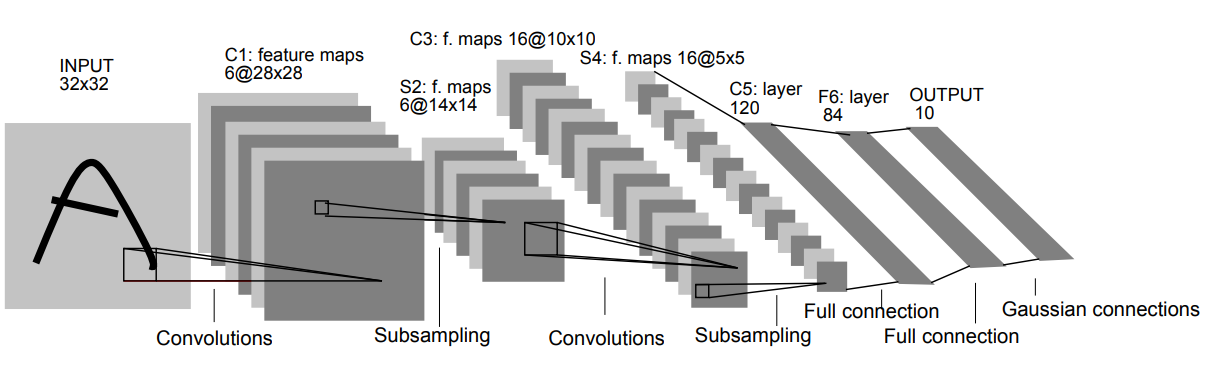
\includegraphics[width=14cm]{img/LeNet-5.png}
    \caption{LeNet-5, CNN for handwritten digits recognition. Source \cite{GradientBasedLearningDigitRec}}
    \label{fig:le-net-5}
\end{figure}

\section{Convolution}
\label{sec:convolution}

Convolution operation on a 3D tensor $H \times W \times D$ (2D image with R, G and B channels) applies a kernel, which is usually a $M \times N \times D$ matrix 
($0 \leq M \leq H, 0 \leq N \leq W$), on the top of spatial location $(0, 0, 0)$. Then products of corresponding elements overlapped by the kernel are computed in all $D$ channels and summed to get the result in this location. The next step is to move move the kernel top to bottom and left to right and perform the convolution operation in every spatial location.

Figure \ref{fig:conv-example} illustrates a convolution on an 2D $4 \times 3$ matrix with an $4 \times 2$ kernel and hopefully clarifies the whole concept. The process for the 3rd order tensor is analogical.

\begin{figure}
    \centering
    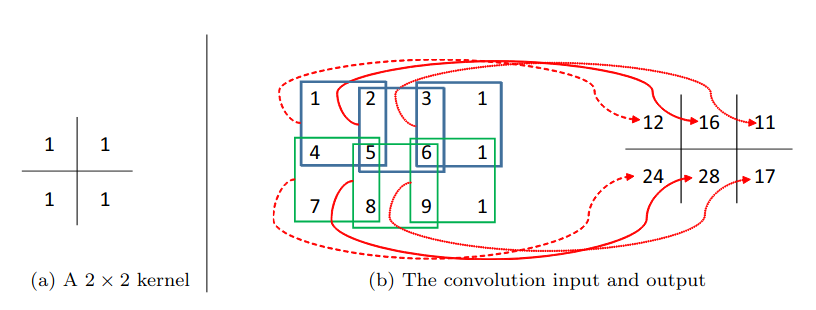
\includegraphics[width=14cm]{img/ConvExample.png}
    \caption{Convolution operation. Source \cite{Wu2017IntroductionTC}}
    \label{fig:conv-example}
\end{figure}

%TODO 6.2 and 6.3 from https://cs.nju.edu.cn/wujx/paper/CNN.pdf

\section{Activation}
\label{sec:conv-activation}

\section{Pooling}
\label{sec:conv-pooling}

\section{Flattening}
\label{sec:flattening}

\section{Full Connection}
\label{sec:full-conn}